\chapter{Conclusions and Future Work}\label{ch:conclusions}

\section{Discussion and Future Work}
Let us introduce possibilities of future work here.

\subsection{Pindakaas}
If we recap the key features of FlashFill \parencite{flashfill} and of TaCLe
\parencite{tacle}, then we would highlight the following:

\textbf{FlashFill}
\begin{itemize}
\item String transformation
\item Marked input-output columns
\item Structured search over programs
\end{itemize}

\textbf{TaCLe}
\begin{itemize}
  \item Textual and numeric flat Excel formulae
  \item Unsupervised
  \item Enumerates all constraints matching the data
\end{itemize}

We see that there indeed possibilities for creating a system that
would take best from two worlds: supervised optimal constraint
learning robust under the noise.

\begin{figure}[htb]
 \centering
 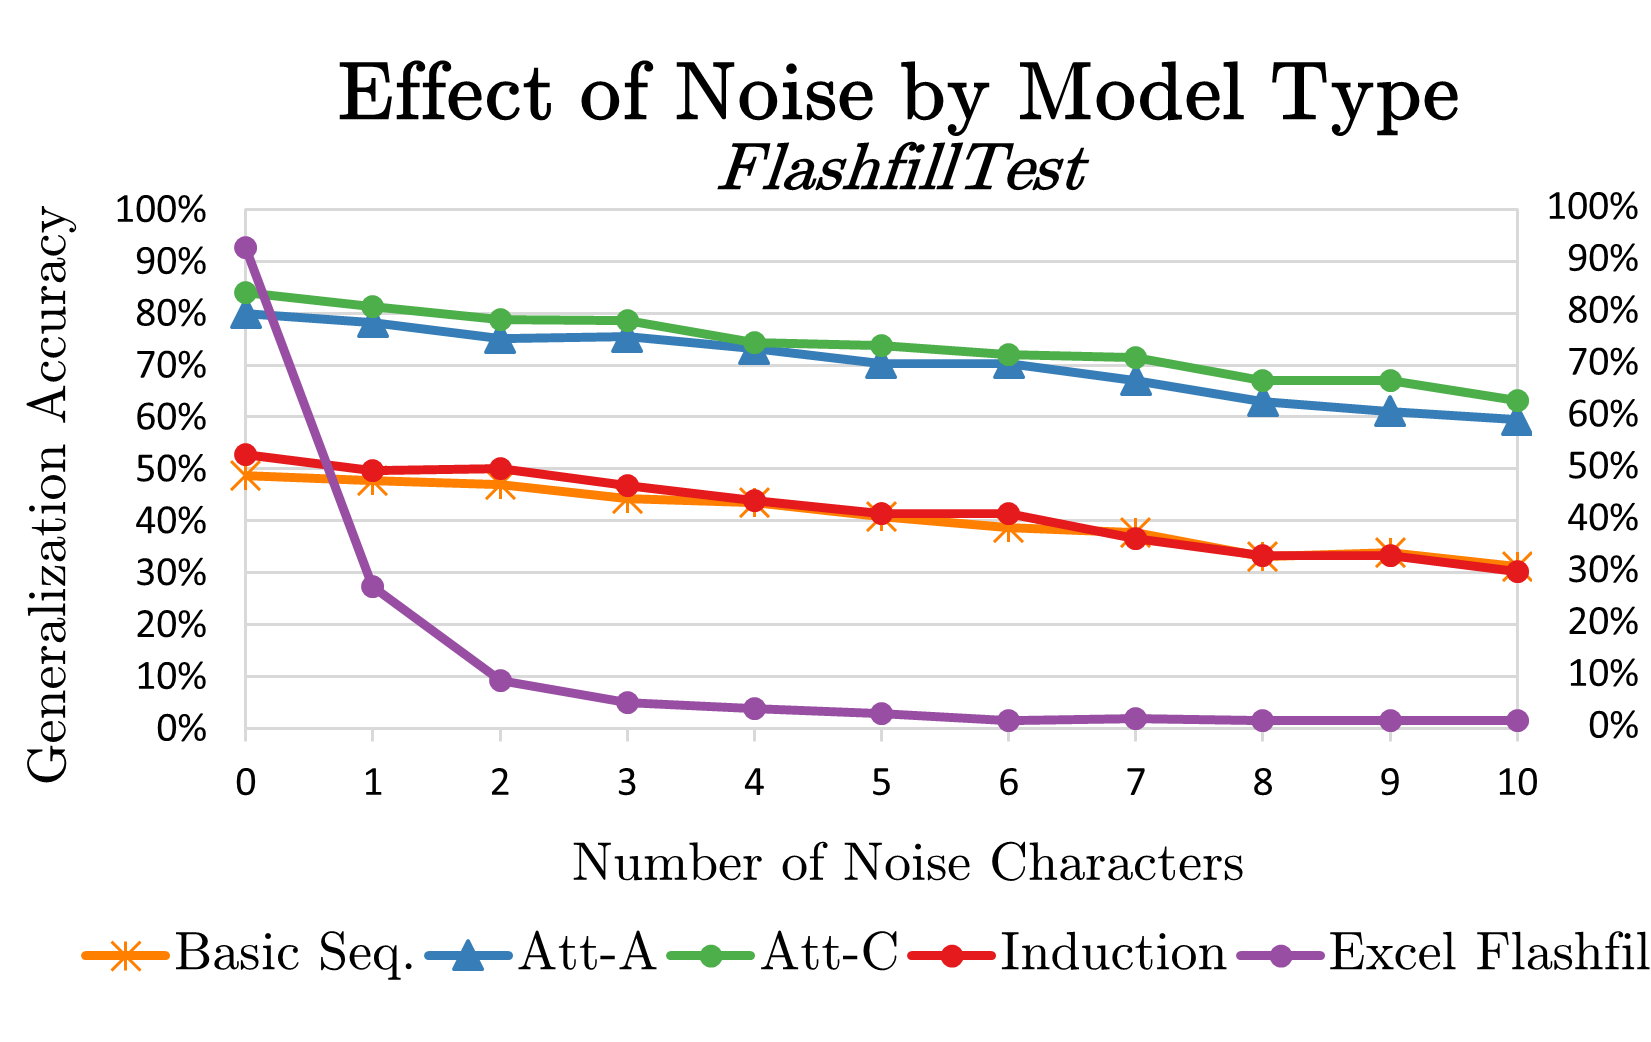
\includegraphics[width=0.7\textwidth]{noise_flashfill.png}
 \caption{We clearly see that FlashFill is highly sensitive to the
   noise (the figure is due to \cite{robustfill})}
  \label{fig:flashfill_noise}
\end{figure}

\begin{figure}[htb]
 \centering
 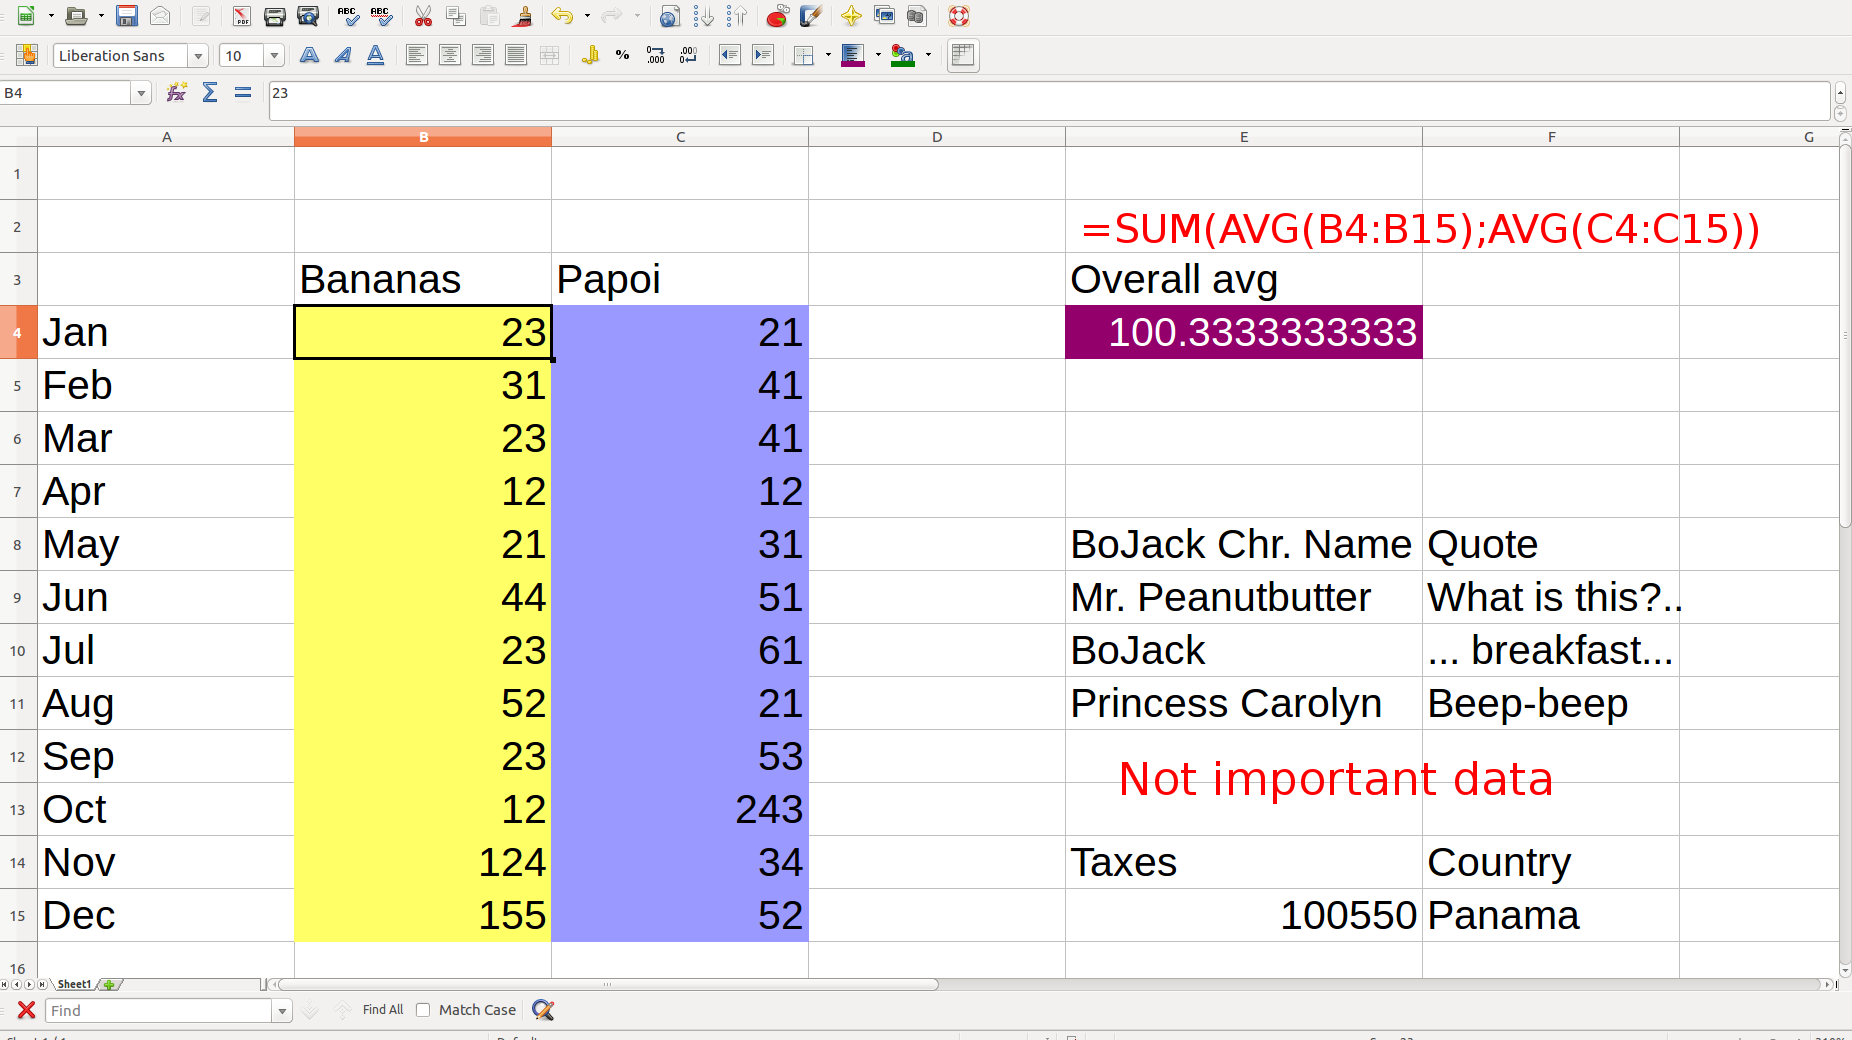
\includegraphics[width=0.7\textwidth]{setting.png}
 \caption{An example of a nested spreadsheet formula}
  \label{fig:nested_formula}
\end{figure}

\begin{figure}[htb]
 \centering
 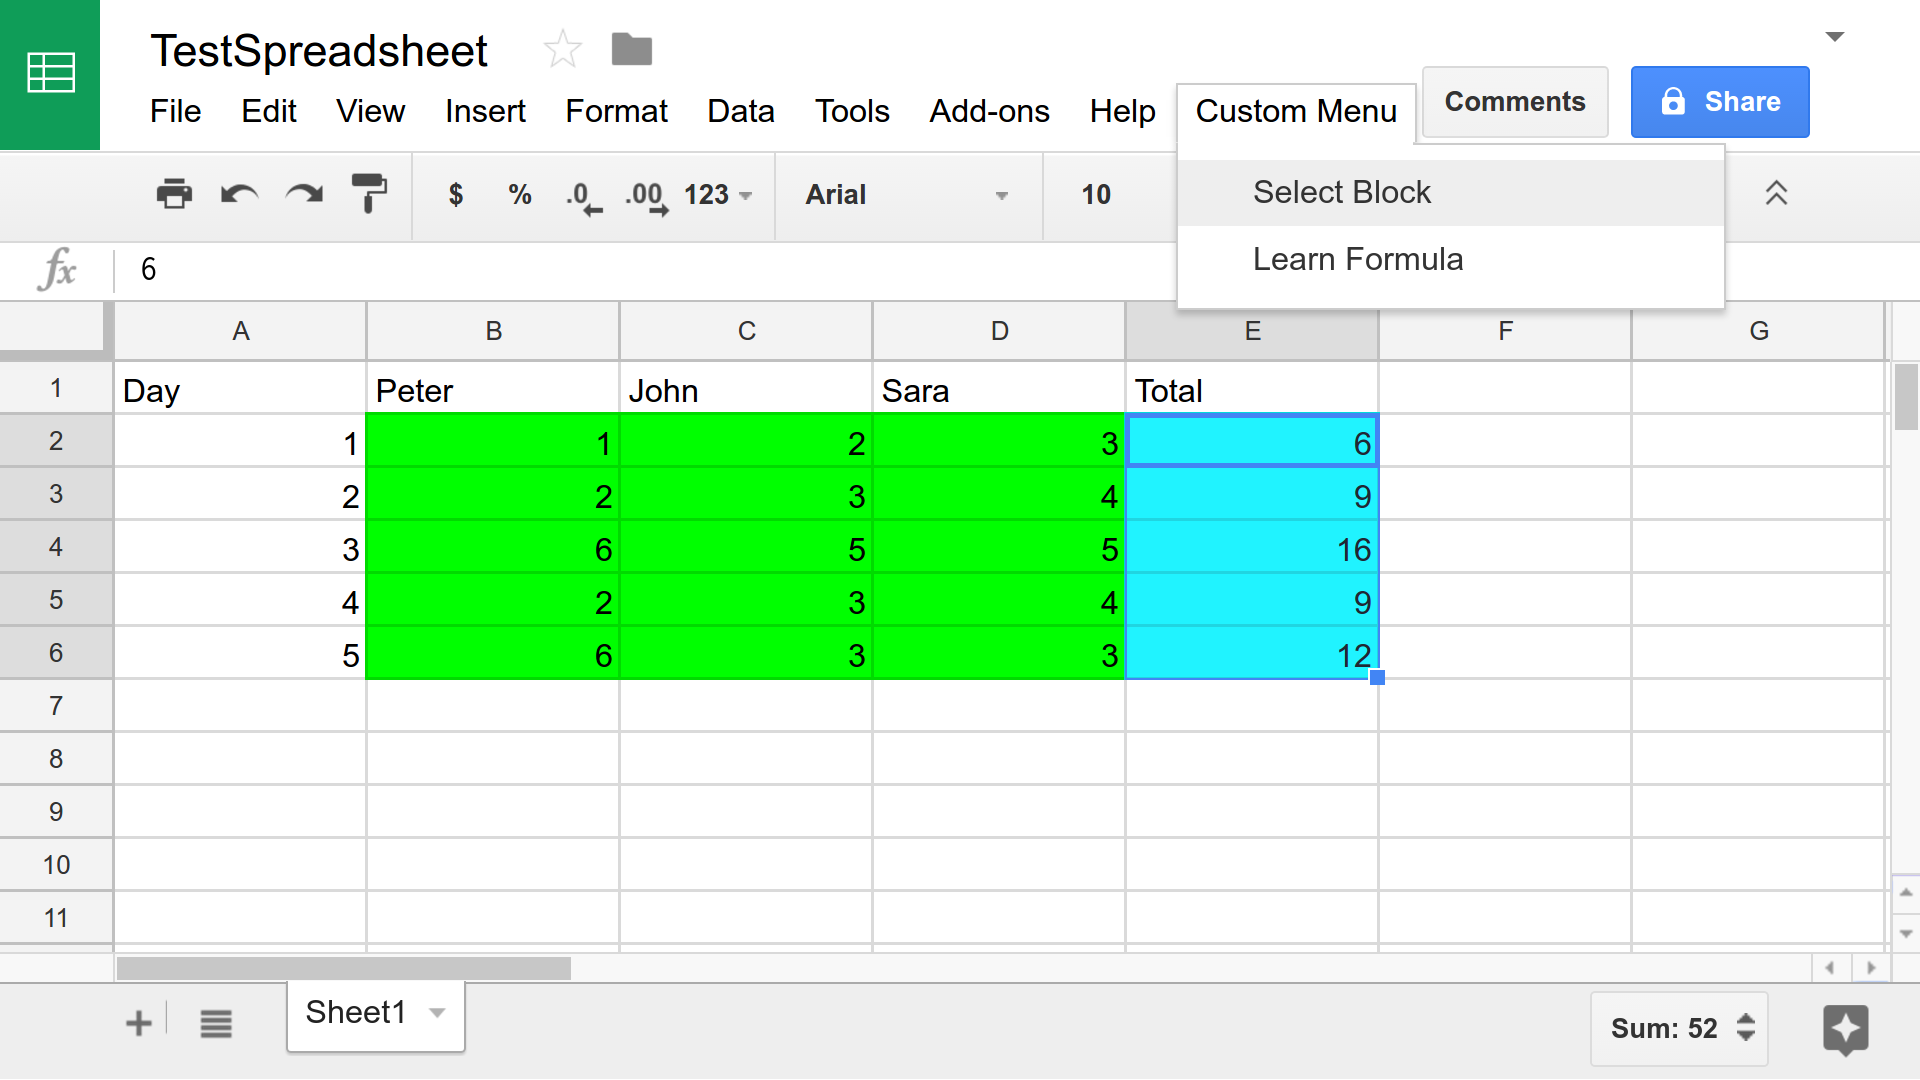
\includegraphics[width=0.7\textwidth]{visualInterface.png}
 \caption{Possible visual interface for Pindakaas}
  \label{fig:visual_interface}
\end{figure}

\textbf{Key Ideas:}
  \begin{itemize}
    \item Use marked or ``supervised'' setting with $\bar x$ for input, $y$ for output
    \item Introduce the loss function $L$ between formula and output
    \item Search for the best fitting formula, i.e., $L(f(\bar x),y)$
    \item Penalize complexity with of a formula, i.e., $\mathcal{C}(f)$ is the measure of complexity
  \end{itemize}




\paragraph{Noise handling} FlashFill is highly sensitive to the noise,
see Figure \ref{fig:flashfill_noise},
and TaCle as well. If we want to make TaCLe robust to the noise, we also need to adapt a
statistical methodology. One way to do it is to introduce a loss
function that would measure how close is the formula to the target
output.

\paragraph{Nested formulae} TaCLe is only able to handle flat
formulae, if we want to extend it to the nested formulae, as for
example in Figure \ref{fig:nested_formula}, we need to
put preference of one formula over another. This can be done by means
of regularizing the formula complexity.

This can be achieved by introducing the following optimization
objective:

  \begin{equation*}
    f^* = \min_{f \in F}{L(f(\bar x),y) + \alpha \mathcal{C}(f)}
  \end{equation*}
  where $\alpha$ is a constant, like in SVM

\paragraph{How can we define complexity}
  \begin{itemize}
     \item for any flat formula $f$, it is a constant
       \begin{equation*}
         \mathcal{C}(f) = c_f 
       \end{equation*}
     \item for any nested formula 
       \begin{equation*}
       \mathcal{C}(f(g(x_1),h(x_2))) = \mathcal{C}(f) + \mathcal{C}(g) + \mathcal{C}(h)
       \end{equation*}
  \end{itemize}
  And the penalization constant $\alpha$ can be learned by cross-validation or set as a parameter

To better position Pindakass, let us contrast it with the features of
TaCLe and FlashFill in Table \ref{tab:pindakaas_features}.
\makesavenoteenv{tabular}
\begin{table}
  \begin{tabularx}{\textwidth}{l | X | X | X }
    \textbf{Property} & \textbf{FlashFill} & \textbf{TaCLe} &
    \textbf{Pindakaas} \\ \hline
    Data type & Text & Numeric and Textual &  Numeric and
    Textual\\\hline
    Learns & String transformation & Set of Flat Excel Formulae
    & Single best nested formula\\\hline
    Supervised & Marked columns + examples & Unsupervised &
    Marked columns \\\hline
    Solving & Structured search & Constraint enumeration &
    Regularized optimization \\\hline
    Satisfaction & Exact & Exact &  Best
    matching\\\hline
    Output & set of values & set of formulae & single
    formula\\ \hline
    Anytime & No & No & Yes
  \end{tabularx}
  \caption{Feature comparison between Pindakaas, TaCLe and FlashFill}
  \label{tab:pindakaas_features}
\end{table}



A possible visual interface is depicted in Figure \ref{fig:visual_interface}.

\subsection{Spreadsheet formula sketching}
Let us suggest a mix between TaCLe and ASP sketching:

\textbf{Problem:} a set of partially specified constraints (or formulae, equations), can we complete them given examples?
 
  Specification (for consistency, Excel-like)
  \begin{verbatim}
  B1 := ?F1(A1:A10)
  B2 := B1 ?+ ?F2(B1)
  B3 := if B2 ?= 10, then ?F3(B2)
                     else 42
  \end{verbatim}
  And examples:
  \begin{verbatim}
  positive: B1 = 4; B2 = 2; B3 = 42 
  negative: B1 = 1; B2 = 2; B3 =  3
  \end{verbatim}
  

  Completed specification that is consistent with the examples:
  \begin{Verbatim}[commandchars=\\\{\}]
  B1 := \textbf{SUM}(A1:A10)
  B2 := B1 \textbf{-} \textbf{SQRT}(B1)
  B3 := if B2 \textbf{>} 10, then B2\textbf{^2}
                    else 42
  \end{Verbatim}

This combines ideas from both \acrshort{skasp} and \acrshort{tacle}.
  

\section{Summary and Conclusions}


%%%%%%%%%%%%%%%%%%%%%%%%%%%%%%%%%%%%%%%%%%%%%%%%%%
% Keep the following \cleardoublepage at the end of this file, 
% otherwise \includeonly includes empty pages.
\cleardoublepage

% vim: tw=70 nocindent expandtab foldmethod=marker foldmarker={{{}{,}{}}}
